\section{Qualidade de Software}

GQM é uma abordagem \textit{top-down} orientado a metas para a mensuração de produtos e processos de software, ou seja, é um processo para definição e interpretação de métricas de software. \cite{junior}

A ideia base desta abordagem é, para cada meta estabelecida dentro da organização identificar questões possíveis de serem respondidas com a análise de medidas coletadas para métricas, sendo a medição então fundamentada em metas que a organização visa alcançar.

O modelo GQM é composto por três níveis:

\begin{figure}[h!]
	\centering
  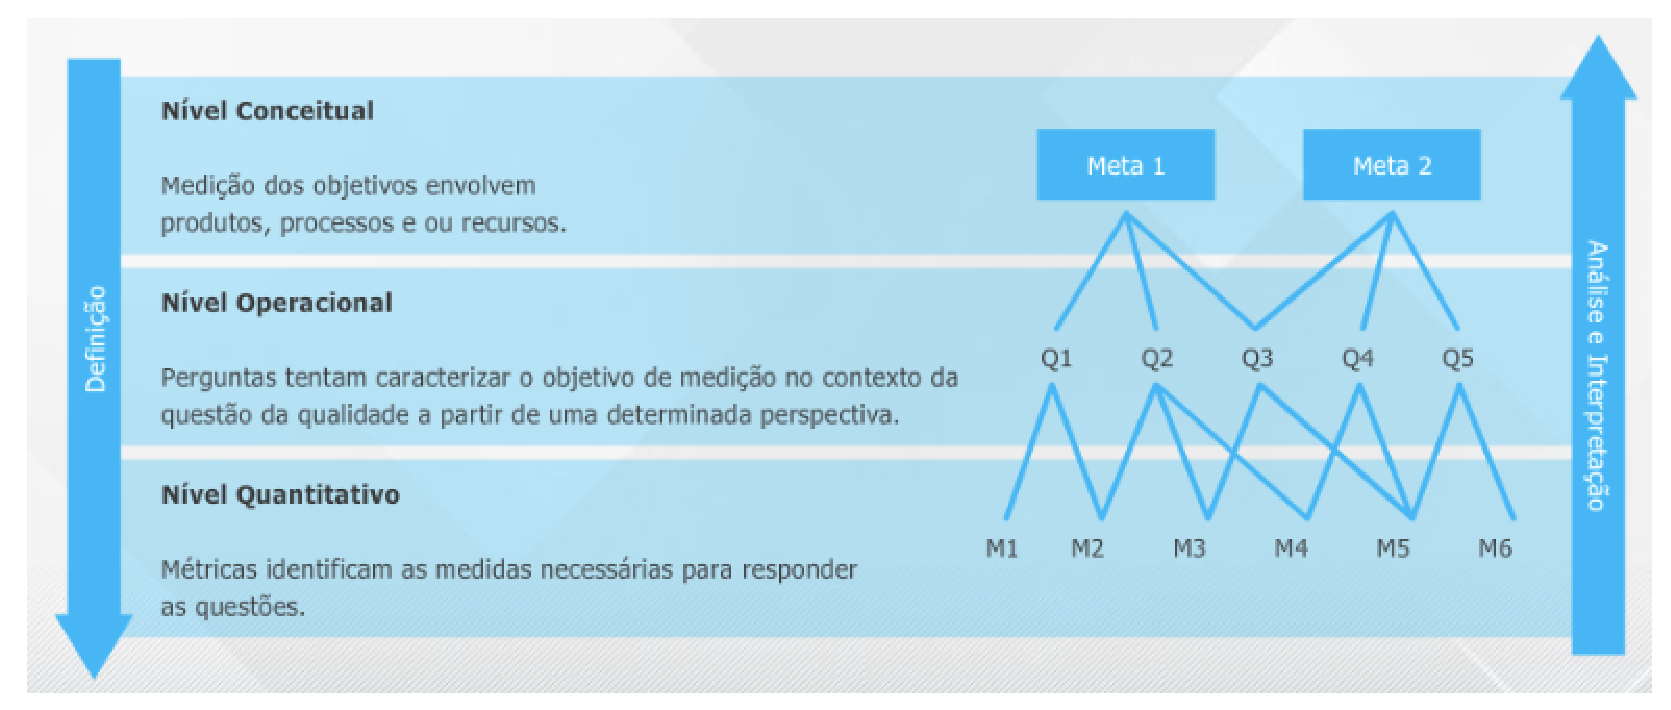
\includegraphics[keepaspectratio=true,scale=0.5]{figuras/gqm.eps}
  \caption{Níveis do GQM. \cite{junior}}
	\label{fig:gqm}
\end{figure}

\begin{itemize}
  \item \textbf{Conceitual}: Uma meta é definida para um objetivo, envolvendo produtos, processos ou recursos.
  \item \textbf{Operacional}: Um conjunto de perguntas é elaborado com relação a cada objetivo identificado.
  \item \textbf{Quantitativo}: Um conjunto de métricas é estabelecido, de maneira a atender a cada pergunta elaborada.
\end{itemize}

Um processo de medição de software direcionado aos objetivos produz medidas que provêem informações para importantes questões de negócio, previamente identificadas. Uma vez que as medidas podem ser rastreadas de volta aos objetivos da organização.
